% Options for packages loaded elsewhere
\PassOptionsToPackage{unicode}{hyperref}
\PassOptionsToPackage{hyphens}{url}
%
\documentclass[
]{article}
\usepackage{lmodern}
\usepackage{amssymb,amsmath}
\usepackage{ifxetex,ifluatex}
\ifnum 0\ifxetex 1\fi\ifluatex 1\fi=0 % if pdftex
  \usepackage[T1]{fontenc}
  \usepackage[utf8]{inputenc}
  \usepackage{textcomp} % provide euro and other symbols
\else % if luatex or xetex
  \usepackage{unicode-math}
  \defaultfontfeatures{Scale=MatchLowercase}
  \defaultfontfeatures[\rmfamily]{Ligatures=TeX,Scale=1}
\fi
% Use upquote if available, for straight quotes in verbatim environments
\IfFileExists{upquote.sty}{\usepackage{upquote}}{}
\IfFileExists{microtype.sty}{% use microtype if available
  \usepackage[]{microtype}
  \UseMicrotypeSet[protrusion]{basicmath} % disable protrusion for tt fonts
}{}
\makeatletter
\@ifundefined{KOMAClassName}{% if non-KOMA class
  \IfFileExists{parskip.sty}{%
    \usepackage{parskip}
  }{% else
    \setlength{\parindent}{0pt}
    \setlength{\parskip}{6pt plus 2pt minus 1pt}}
}{% if KOMA class
  \KOMAoptions{parskip=half}}
\makeatother
\usepackage{xcolor}
\IfFileExists{xurl.sty}{\usepackage{xurl}}{} % add URL line breaks if available
\IfFileExists{bookmark.sty}{\usepackage{bookmark}}{\usepackage{hyperref}}
\hypersetup{
  pdftitle={Microarray Analysis PAC1},
  pdfauthor={David Cartoixà Cartoixà},
  hidelinks,
  pdfcreator={LaTeX via pandoc}}
\urlstyle{same} % disable monospaced font for URLs
\usepackage[margin=1in]{geometry}
\usepackage{color}
\usepackage{fancyvrb}
\newcommand{\VerbBar}{|}
\newcommand{\VERB}{\Verb[commandchars=\\\{\}]}
\DefineVerbatimEnvironment{Highlighting}{Verbatim}{commandchars=\\\{\}}
% Add ',fontsize=\small' for more characters per line
\usepackage{framed}
\definecolor{shadecolor}{RGB}{248,248,248}
\newenvironment{Shaded}{\begin{snugshade}}{\end{snugshade}}
\newcommand{\AlertTok}[1]{\textcolor[rgb]{0.94,0.16,0.16}{#1}}
\newcommand{\AnnotationTok}[1]{\textcolor[rgb]{0.56,0.35,0.01}{\textbf{\textit{#1}}}}
\newcommand{\AttributeTok}[1]{\textcolor[rgb]{0.77,0.63,0.00}{#1}}
\newcommand{\BaseNTok}[1]{\textcolor[rgb]{0.00,0.00,0.81}{#1}}
\newcommand{\BuiltInTok}[1]{#1}
\newcommand{\CharTok}[1]{\textcolor[rgb]{0.31,0.60,0.02}{#1}}
\newcommand{\CommentTok}[1]{\textcolor[rgb]{0.56,0.35,0.01}{\textit{#1}}}
\newcommand{\CommentVarTok}[1]{\textcolor[rgb]{0.56,0.35,0.01}{\textbf{\textit{#1}}}}
\newcommand{\ConstantTok}[1]{\textcolor[rgb]{0.00,0.00,0.00}{#1}}
\newcommand{\ControlFlowTok}[1]{\textcolor[rgb]{0.13,0.29,0.53}{\textbf{#1}}}
\newcommand{\DataTypeTok}[1]{\textcolor[rgb]{0.13,0.29,0.53}{#1}}
\newcommand{\DecValTok}[1]{\textcolor[rgb]{0.00,0.00,0.81}{#1}}
\newcommand{\DocumentationTok}[1]{\textcolor[rgb]{0.56,0.35,0.01}{\textbf{\textit{#1}}}}
\newcommand{\ErrorTok}[1]{\textcolor[rgb]{0.64,0.00,0.00}{\textbf{#1}}}
\newcommand{\ExtensionTok}[1]{#1}
\newcommand{\FloatTok}[1]{\textcolor[rgb]{0.00,0.00,0.81}{#1}}
\newcommand{\FunctionTok}[1]{\textcolor[rgb]{0.00,0.00,0.00}{#1}}
\newcommand{\ImportTok}[1]{#1}
\newcommand{\InformationTok}[1]{\textcolor[rgb]{0.56,0.35,0.01}{\textbf{\textit{#1}}}}
\newcommand{\KeywordTok}[1]{\textcolor[rgb]{0.13,0.29,0.53}{\textbf{#1}}}
\newcommand{\NormalTok}[1]{#1}
\newcommand{\OperatorTok}[1]{\textcolor[rgb]{0.81,0.36,0.00}{\textbf{#1}}}
\newcommand{\OtherTok}[1]{\textcolor[rgb]{0.56,0.35,0.01}{#1}}
\newcommand{\PreprocessorTok}[1]{\textcolor[rgb]{0.56,0.35,0.01}{\textit{#1}}}
\newcommand{\RegionMarkerTok}[1]{#1}
\newcommand{\SpecialCharTok}[1]{\textcolor[rgb]{0.00,0.00,0.00}{#1}}
\newcommand{\SpecialStringTok}[1]{\textcolor[rgb]{0.31,0.60,0.02}{#1}}
\newcommand{\StringTok}[1]{\textcolor[rgb]{0.31,0.60,0.02}{#1}}
\newcommand{\VariableTok}[1]{\textcolor[rgb]{0.00,0.00,0.00}{#1}}
\newcommand{\VerbatimStringTok}[1]{\textcolor[rgb]{0.31,0.60,0.02}{#1}}
\newcommand{\WarningTok}[1]{\textcolor[rgb]{0.56,0.35,0.01}{\textbf{\textit{#1}}}}
\usepackage{longtable,booktabs}
% Correct order of tables after \paragraph or \subparagraph
\usepackage{etoolbox}
\makeatletter
\patchcmd\longtable{\par}{\if@noskipsec\mbox{}\fi\par}{}{}
\makeatother
% Allow footnotes in longtable head/foot
\IfFileExists{footnotehyper.sty}{\usepackage{footnotehyper}}{\usepackage{footnote}}
\makesavenoteenv{longtable}
\usepackage{graphicx,grffile}
\makeatletter
\def\maxwidth{\ifdim\Gin@nat@width>\linewidth\linewidth\else\Gin@nat@width\fi}
\def\maxheight{\ifdim\Gin@nat@height>\textheight\textheight\else\Gin@nat@height\fi}
\makeatother
% Scale images if necessary, so that they will not overflow the page
% margins by default, and it is still possible to overwrite the defaults
% using explicit options in \includegraphics[width, height, ...]{}
\setkeys{Gin}{width=\maxwidth,height=\maxheight,keepaspectratio}
% Set default figure placement to htbp
\makeatletter
\def\fps@figure{htbp}
\makeatother
\setlength{\emergencystretch}{3em} % prevent overfull lines
\providecommand{\tightlist}{%
  \setlength{\itemsep}{0pt}\setlength{\parskip}{0pt}}
\setcounter{secnumdepth}{-\maxdimen} % remove section numbering
\usepackage{booktabs}
\usepackage{longtable}
\usepackage{array}
\usepackage{multirow}
\usepackage{wrapfig}
\usepackage{float}
\usepackage{colortbl}
\usepackage{pdflscape}
\usepackage{tabu}
\usepackage{threeparttable}
\usepackage{threeparttablex}
\usepackage[normalem]{ulem}
\usepackage{makecell}
\usepackage{xcolor}

\title{Microarray Analysis PAC1}
\author{David Cartoixà Cartoixà}
\date{April 18,2020}

\begin{document}
\maketitle

\textbf{INDICE DE CONTENIDOS}

1.\protect\hyperlink{id1}{Abstract} 2.\protect\hyperlink{id2}{Objetivo
del estudio y datos} 2.1.\protect\hyperlink{id3}{Objetivos del estudio}
2.2.\protect\hyperlink{id4}{Obtención de las muestras} 2.3.
\protect\hyperlink{id5}{Análisis de microarrays}
3.\protect\hyperlink{id6}{Métodos}
3.1.\protect\hyperlink{id7}{Preparación del entorno de trabajo}
3.2.\protect\hyperlink{id8}{Preparación de los datos para el análisis}
3.3.\protect\hyperlink{id9}{Instalación de paquetes en R}
3.4.\protect\hyperlink{id10}{Lectura de los archivos .CEL}
3.5.\protect\hyperlink{id11}{Control de calidad de los datos sin
procesar} 3.6.\protect\hyperlink{id12}{Control de calidad de los datos
procesados} 3.7.\protect\hyperlink{id13}{Análisis de batch}
3.8.\protect\hyperlink{id14}{Detección de los genes más variables}
3.9.\protect\hyperlink{id15}{Filtrado de genes}
3.10.\protect\hyperlink{id16}{Guardado de los datos normalizados y
filtrados} 3.11.\protect\hyperlink{id17}{Definición de la matriz de
diseño} 3.12.\protect\hyperlink{id18}{Definición de la matriz de
contrastes} 3.13.\protect\hyperlink{id19}{Estimación del modelo y
selección de genes} 3.14.\protect\hyperlink{id20}{Obtención de una lista
de genes expresados diferencialmente}
3.15.\protect\hyperlink{id21}{Anotación genética}
3.16.\protect\hyperlink{id22}{Visualización de la expresión diferencial}
3.17.\protect\hyperlink{id23}{Comparaciones múltiples}
3.18.\protect\hyperlink{id24}{Heatmaps}
3.19.\protect\hyperlink{id25}{Significación biológica de los resultados}
4.\protect\hyperlink{id26}{Código R}
5.\protect\hyperlink{id27}{Referencias}

El siguiente informe y sus datos se pueden consultar en
\url{https://github.com/dcc1978/Statistical-Analysis-of-Microarray-Data-PEC1/}

\hypertarget{abstract}{%
\section{1.Abstract}\label{abstract}}

El factor de crecimiento transformante \(\beta1\) (\(TGF\beta1\)) es una
citocina implicada en el control y la diferenciación celular, la
desregulaciónn de la activación y de la ruta de señalización de
(\(TGF\beta1\)) puede desencadednar apoptosis.Se ha demostrado que la
CAV1 o caveolina-1, que es una proteina transmembrana, altera la
señalización de (\(TGF\beta1\)).En el estudio se utilizaron hepatocitos
estimulados con el factor de crecimiento en ratones normales y en
ratones knock-out para caveolina.

\hypertarget{palabras-clave}{%
\section{Palabras clave}\label{palabras-clave}}

Caveolina-1, factor de crecimiento transformante \(\beta1\),
metabolismo, enfermedades hepáticas, microarray

\hypertarget{objetivos-del-estudio-y-datos}{%
\section{2.Objetivos del estudio y
datos}\label{objetivos-del-estudio-y-datos}}

\hypertarget{objetivos-del-estudio}{%
\subsection{2.1.Objetivos del estudio}\label{objetivos-del-estudio}}

El objetivo del estudio es evaluar si el papel de la caveolina-1 sobre
afecta el control de los gene signature inducidos por el factor de
crecimiento transformante \(\beta1\), en consecuencia se pretende un
mejor conocimiento de la función de (\(TGF\beta1\)) en hígado sano y en
hígado enfermo, donde los niveles de CAV1 se encuentran implicados.

\hypertarget{obtenciuxf3n-de-las-muestras}{%
\subsection{2.2. Obtención de las
muestras}\label{obtenciuxf3n-de-las-muestras}}

\begin{itemize}
\tightlist
\item
  Se utilizaron cuatro grupos de hepatocitos de ratón C57BL/6 de doce
  semanas de edad:

  \begin{itemize}
  \tightlist
  \item
    Grupo 1: cultivado con CAV1 y con \(TGF\beta1\).
  \item
    Grupo 2: cultivado con CAv1.
  \item
    Grupo 3: cultivado con \(TGF\beta1\).
  \item
    Grupo 4: grupo control.
  \end{itemize}
\end{itemize}

\hypertarget{anuxe1lisis-de-microarrays}{%
\subsection{2.3 Análisis de
microarrays}\label{anuxe1lisis-de-microarrays}}

Para analizar las diferencias de expresión génica con los diferentes
tratamientos se utilizaron 12 arrays de Affymetrix MoGene 2.0, 3 para
cada uno de los grupos mencionados en el apartado anterior. Los datos
que hemos empleado en el estudio se encuentran disponibles en la bse de
datos Gene Expresion Omnibus (GEO), perteneciente al NCBI y disponibles
con el número de acceso
GSE137339(\url{https://www.ncbi.nlm.nih.gov/geo/download/?acc=GSE137339}).

\hypertarget{muxe9todos}{%
\section{3. Métodos}\label{muxe9todos}}

\hypertarget{preparaciuxf3n-del-entorno-de-trabajo}{%
\subsection{3.1 Preparación del entorno de
trabajo}\label{preparaciuxf3n-del-entorno-de-trabajo}}

Primeramente definiremos el directorio de trabajo, y crearemos tres
carpetas: ``data'' donde almacenaremos los archivos .CEL descomprimidos
y los archivos generados por nosotros target; una carpeta ``results''
donde registraremos los resultados obtenidos y finalmente la carpeta
``figures'' en la cual almacenaremos las figuras del estudio.

\begin{Shaded}
\begin{Highlighting}[]
\OperatorTok{>}\StringTok{ }\KeywordTok{setwd}\NormalTok{(}\StringTok{"."}\NormalTok{)}
\OperatorTok{>}\StringTok{ }\KeywordTok{dir.create}\NormalTok{(}\StringTok{"data"}\NormalTok{)}
\OperatorTok{>}\StringTok{ }\KeywordTok{dir.create}\NormalTok{(}\StringTok{"results"}\NormalTok{)}
\OperatorTok{>}\StringTok{ }\KeywordTok{dir.create}\NormalTok{(}\StringTok{"figures"}\NormalTok{)}
\end{Highlighting}
\end{Shaded}

\hypertarget{preparaciuxf3n-de-los-datos-para-el-anuxe1lisis}{%
\subsection{3.2 Preparación de los datos para el
análisis}\label{preparaciuxf3n-de-los-datos-para-el-anuxe1lisis}}

Los datos para el análisis constan de dos tipos de archivo, los archivos
``CEL''(en nuestro caso 12 archivos .CEL que hemos descargado), y un
archivo ``targets.xlsx'' que posteriormente convertimos a
``targets.csv''. Los archivos ``CEL'' son los datos sin procesar
originados después de escanear y preprocesar el microarray con el
software Affymetrix. Los archivos mencionados los almacenaremos en la
carpeta ``data''. El archivo ``targets'' contiene la información sobre
grupos y covariables, relaciona el nombre de cada archivo .CEL con su
condición en el experimento.

Para el análisis el archivo targets ha sido guardado con formato .csv,
hemos creado el archivo a raíz de la información obtenida en
(\url{https://www.ncbi.nlm.nih.gov/geo/query/acc.cgi?acc=GSE137339}). La
tabla 1 muestra el contenido del archivo ``targets'' utilizado en el
presente análisis:

\begin{longtable}[]{@{}llllll@{}}
\caption{Tabla1. Contenido del fichero targets utilizados para el
análisis}\tabularnewline
\toprule
Accession & Title & Sirma & Treatment & ShortName & Group\tabularnewline
\midrule
\endfirsthead
\toprule
Accession & Title & Sirma & Treatment & ShortName & Group\tabularnewline
\midrule
\endhead
GSM4075756 & siCav1+TGF-Beta1 rep1 & Caveolin-1 & TGFBeta & Cav1.TGFB1 &
Cav.TGFB1\tabularnewline
GSM4075757 & siCav1+TGF-Beta1 rep2 & Caveolin-1 & TGFBeta & Cav1.TGFB2 &
Cav.TGFB1\tabularnewline
GSM4075758 & siCav1+TGF-Beta1 rep3 & Caveolin-1 & TGFBeta & Cav1.TGFB3 &
Cav.TGFB1\tabularnewline
GSM4075759 & siCAV1 rep1 & Caveolin-1 & Ctrl & Cav1.Ctrl1 &
Cav.Ctrl\tabularnewline
GSM4075760 & siCAV1 rep 2 & Caveolin-1 & Ctrl & Cav1.Ctrl2 &
Cav.Ctrl\tabularnewline
GSM4075761 & siCAV1 rep 3 & Caveolin-1 & Ctrl & Cav1.Ctrl3 &
Cav.Ctrl\tabularnewline
GSM4075762 & siCon+TGF-Beta1 rep 1 & Ctrl & TGFBeta & Con1.TGFB1 &
Con.TGFB1\tabularnewline
GSM4075763 & siCon+TGF-Beta1 rep 2 & Ctrl & TGFBeta & Con1.TGFB2 &
Con.TGFB1\tabularnewline
GSM4075764 & siCon+TGF-Beta1 rep 3 & Ctrl & TGFBeta & Con1.TGFB3 &
Con.TGFB1\tabularnewline
GSM4075765 & siCon rep 1 & Ctrl & Ctrl & Con1.Ctrl1 &
Con.Ctrl\tabularnewline
GSM4075766 & siCon rep 2 & Ctrl & Ctrl & Con1.Ctrl2 &
Con.Ctrl\tabularnewline
GSM4075767 & siCon rep 3 & Ctrl & Ctrl & Con1.Ctrl3 &
Con.Ctrl\tabularnewline
\bottomrule
\end{longtable}

\hypertarget{instalaciuxf3n-de-paquetes-en-r}{%
\subsection{3.3 Instalación de paquetes en
R}\label{instalaciuxf3n-de-paquetes-en-r}}

Los paquetes no disponibles en la instalación básica de R deben
instalarse antes de proceder con el análisis. Los paquetes necesarios
para realizar el estudio se pueden descargar de distintos repositorios,
los más comunes serán CRAN para paquetes estándar o Bioconductor. Los
paquetes r estándar se pueden descargar e instalar repositorios
predeterminados de formulario con la función install.packages. Los
envases de bioconductor se pueden descargar e instalar con la función
biocLite() que en su momento se puede cargar en R con la fuente de
instrucciones(``\url{https://bioconductor.org/biocLite.R}'').\\
El siguiente código descargará e instalará los paquetes necesarios para
el análisis. Éste código debe ejecutarse solo una vez. Las ejecuciones
posteriores del análisis no necesitan volver a instalar los paquetes.

\hypertarget{lectura-de-los-archivos-cel}{%
\subsection{3.4. Lectura de los archivos
CEL}\label{lectura-de-los-archivos-cel}}

El siguiente paso es leer los datos sin procesar (archivos .CEL) y
almacenar los datos en una variable (en este caso lo hemos llamado
rawData). Primero tenemos que cargar el paquete oligo con la biblioteca
de funciones. En este paquete se codifican las funciones para leer los
archivos CEL.

\begin{verbatim}
Reading in : ./data/GSM4075756_Meyer_270213_6-sicav_+48h_TGFbeta-I_MoGene-1_0-st-v1_.CEL
Reading in : ./data/GSM4075757_Meyer_270213_12-sicav_+48h_TGFbeta-III_MoGene-1_0-st-v1_.CEL
Reading in : ./data/GSM4075758_Meyer_270213_18-sicav_+48h_TGFbeta-IV_MoGene-1_0-st-v1_.CEL
Reading in : ./data/GSM4075759_Meyer_270213_4-sicav_48h-I_MoGene-1_0-st-v1_.CEL
Reading in : ./data/GSM4075760_Meyer_270213_10-sicav_48h-III_MoGene-1_0-st-v1_.CEL
Reading in : ./data/GSM4075761_Meyer_270213_16-sicav_48h-IV_MoGene-1_0-st-v1_.CEL
Reading in : ./data/GSM4075762_Meyer_270213_5-sico_+48h_TGFbeta-I_MoGene-1_0-st-v1_2.CEL
Reading in : ./data/GSM4075763_Meyer_270213_11-sico_+48h_TGFbeta-III_MoGene-1_0-st-v1_.CEL
Reading in : ./data/GSM4075764_Meyer_270213_17-sico_+48h_TGFbeta-IV_MoGene-1_0-st-v1_.CEL
Reading in : ./data/GSM4075765_Meyer_270213_3-sico_48h-I_MoGene-1_0-st-v1_.CEL
Reading in : ./data/GSM4075766_Meyer_270213_9-sico_48h-III_MoGene-1_0-st-v1_.CEL
Reading in : ./data/GSM4075767_Meyer_270213_15-sico_48h-IV_MoGene-1_0-st-v1_.CEL
\end{verbatim}

Para facilitar nuestro trabajo, cambiaremos el nombre largo por las
abreviaturas asignadas (ShortName):

\begin{Shaded}
\begin{Highlighting}[]
\OperatorTok{>}\StringTok{ }\KeywordTok{colnames}\NormalTok{(rawData) <-}\KeywordTok{rownames}\NormalTok{(}\KeywordTok{pData}\NormalTok{(rawData)) <-}\StringTok{ }\NormalTok{my.targets}\OperatorTok{@}\NormalTok{data}\OperatorTok{$}\NormalTok{ShortName}
\end{Highlighting}
\end{Shaded}

\hypertarget{control-de-calidad-de-los-datos-sin-procesar}{%
\subsection{3.5.Control de calidad de los datos sin
procesar}\label{control-de-calidad-de-los-datos-sin-procesar}}

Empleamos la libreria ``arrayQualityMetrics()'' para realizar el control
de calidad de los raw data. Comprobamos los resultados del análisis de
calidad en una carpeta QCDIR.raw creada dntro de la carpeta de resultado
creada anteriormente. Dentro de ésta carpeta buscaremos un archivo
llamado index.html, que abre una página web desde donde podremos acceder
a un resumen del análisis realizado. La figura 1 muestra el encabezado
de éste archivo que contiene una tabla con tres columnas que indican
algunos criterios de calidad que deben ser verificados. Se han marcado 5
muestras, generlamente si sólo hay una marca significa que los problemas
potenciales que pueden acarrear son pequeños, por lo que podemos decidir
mantener todas las muestras en el análisis.

\begin{Shaded}
\begin{Highlighting}[]
\OperatorTok{>}\StringTok{ }\KeywordTok{require}\NormalTok{(arrayQualityMetrics)}
\OperatorTok{>}\StringTok{ }\KeywordTok{arrayQualityMetrics}\NormalTok{(rawData, }\DataTypeTok{outdir =} \KeywordTok{file.path}\NormalTok{(}\StringTok{"./results"}\NormalTok{, }\StringTok{"QCDir.Raw"}\NormalTok{), }\DataTypeTok{force=}\OtherTok{TRUE}\NormalTok{)}
\end{Highlighting}
\end{Shaded}

\begin{figure}

{\centering 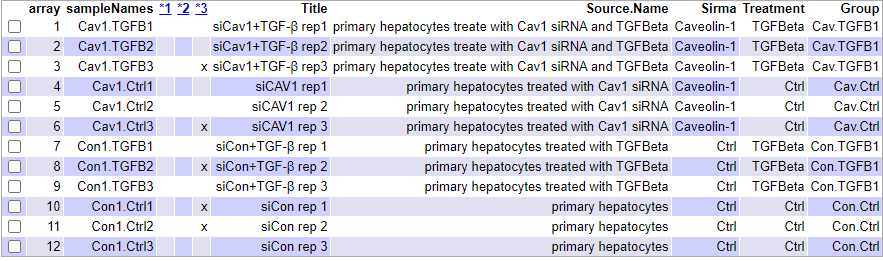
\includegraphics[width=12.26in]{figures/figura1} 

}

\caption{Figura1. Resumen del control de calidad de los datos crudos producido por arrayQualityMetrics()}\label{fig:QCRawDataRes}
\end{figure}

Realizaremos otro análisis de calidad, el análisis de componentes
principales (PCA Analysis) y generando su gráfica, la cual podemos
apreciar en la figura 2.

\begin{figure}

{\centering \includegraphics{cartoixa_david_ADO_PEC1_files/figure-latex/PCARaw-1} 

}

\caption{Figura 2.Visualización de los componentes principales de los datos sin procesar}\label{fig:PCARaw}
\end{figure}

El primer componente del PCA abarca un total del 49.3\% de la
variabilidad de las muestras,y el segundo abarca un 25.2\%. Podemos
deducir que la variabilidad está condicionada al tipo de tratamiento, ya
que en el análisis se observa claramente como los grupos se diferencian
al estar tratados con el factor de crecimiento o sin él.

Realizamos una figura de la distribuión de las intensidades mediante un
``boxplot''en la figura 3, donde observamos una ligera variación de las
intensidades entre arrays, pero es lo esperado para los datos sin
procesar. Cada color representa a un grupo de datos.

\begin{figure}

{\centering \includegraphics{cartoixa_david_ADO_PEC1_files/figure-latex/BoxplotRaw-1} 

}

\caption{Figura 3.Boxplot de los datos sin procesar}\label{fig:BoxplotRaw}
\end{figure}

\hypertarget{control-de-calidad-de-los-datos-procesados}{%
\subsection{3.6. Control de calidad de los datos
procesados}\label{control-de-calidad-de-los-datos-procesados}}

Antes de emprender el análisis de la expresión diferencial, necesitamos
optimizar los arrays y que sean comparables entre ellos, reduciendo y si
es posible eliminando, toda la variabilidad de las muestras que no son
debidas a razones biológicas. Queremos pues, asegurarnos que las
diferencias son debidas a la expresión diferencial de los genes y no a
sesgos artificiales debidos a problemas técnicos.

Volvemos a realizar un control de los datos normalizados para
compararlos con los rawdata

\begin{Shaded}
\begin{Highlighting}[]
\OperatorTok{>}\StringTok{ }\KeywordTok{library}\NormalTok{(arrayQualityMetrics)}
\OperatorTok{>}\StringTok{ }\KeywordTok{arrayQualityMetrics}\NormalTok{(eset_rma,}\DataTypeTok{outdir=}\KeywordTok{file.path}\NormalTok{(}\StringTok{"./results/QCDir.Norm"}\NormalTok{),}\DataTypeTok{force=}\OtherTok{TRUE}\NormalTok{)}
\end{Highlighting}
\end{Shaded}

Los resultados obtenidos de arrayQualityMetrics nos muestrasn una
notable mejora de los indicadores

\begin{figure}

{\centering 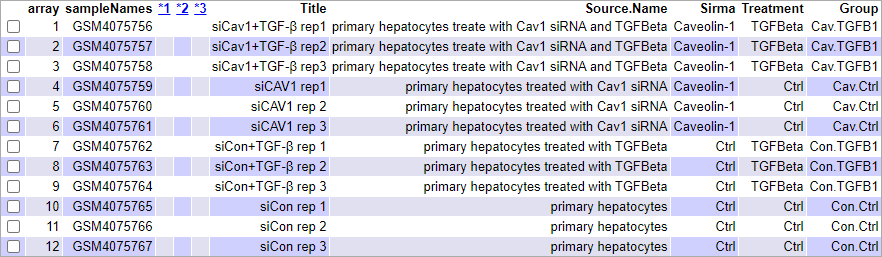
\includegraphics[width=1\linewidth]{figures/figura4} 

}

\caption{Figura4. Resumen de resultados del control de calidad para de los datos normalizados}\label{fig:control de calidad de datos normalizados resultados}
\end{figure}

La figura 4 muestra el mismo resumen que el mostrado anteriormente, pero
se realiza con datos normalizados. Obsérvese que ya no hay ninguna
columna marcada.

Realizamos un gráfico del análisis de los componentes principales
realizados en datos normalizados:

\begin{figure}

{\centering \includegraphics{cartoixa_david_ADO_PEC1_files/figure-latex/PCANorm-1} 

}

\caption{Figura 5.Visualización de los componentes principales de los datos normalizados}\label{fig:PCANorm}
\end{figure}

En la figura 5 vemos que el primer componente representa el 57.5\% de la
variabilidad total, el porcentaje de variabilidad explicada ha aumentado
con respecto al análisis anterior en datos sin procesar. Del mismo modo
que con el PCA con datos sin procesar, separa las muestra de la
condición sin TGFB1 a la derecha y las muestras tratadas con TGFB1 a la
izquierda.

Volvemos a diseñar un boxplot pero esta vez con los datos normalizados
para contrastarlos con el boxplot anterior.

\begin{figure}

{\centering \includegraphics{cartoixa_david_ADO_PEC1_files/figure-latex/BoxplotNorm-1} 

}

\caption{Figura 6. Boxplot de los datos normalizados}\label{fig:BoxplotNorm}
\end{figure}

En la figura 6 se observa una gráfica boxplot que representa la
distribución de las intensidades normalizadas a lo largo de todas las
muestras con los datos normalizados, sugiere que la normalización ha
funcionado correctamente.

Como una siguiente observación al análisis de normalización, haremos una
comparativa de los gráficos ``MA-plot'', haciendo una comparativa de los
gráficos que corresponden a las muestras sin procesar (figura 7) y a las
muestras normalizadas (figura 8). Observamos que los datos se centran a
lo largo del eje M=0, que es lo que esperabamos.

\begin{figure}

{\centering 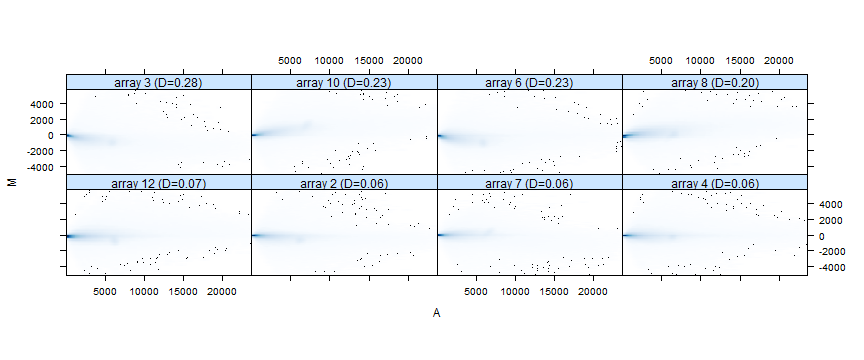
\includegraphics[width=1\linewidth]{figures/maraw} 

}

\caption{Figura 7.MA plot de los datos sin procesar}\label{fig:control de calidad de datos MAplot raw}
\end{figure}

\begin{figure}

{\centering 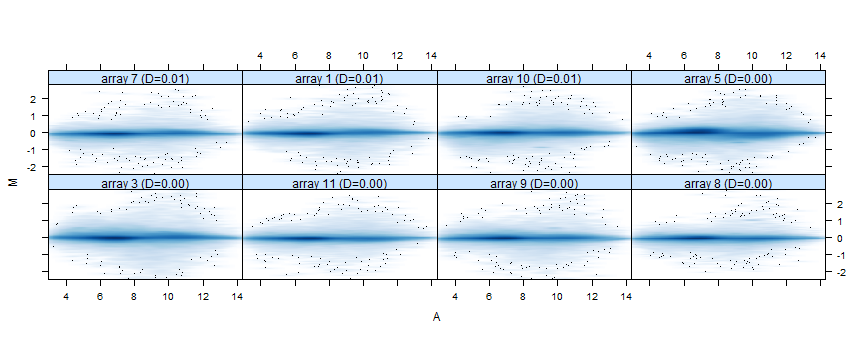
\includegraphics[width=1\linewidth]{figures/manorm} 

}

\caption{Figura 8.MA plot de los datos normalizados}\label{fig:control de calidad de datos MAnorm}
\end{figure}

\hypertarget{anuxe1lisis-de-batch}{%
\subsection{3.7. Análisis de batch}\label{anuxe1lisis-de-batch}}

Los resultados de los microarrays de expresión génica pueden verse
afectados por diferencias minúsculas en cualquier número de variables no
biológicas como reactivos de diferentes lotes, la manipulación de
técnicos diferentes y la más habitual que es la diferente fecha de
procesamiento de las muestras del mismo experimento. El error
acumulativo introducido por éstas variaciones experimentales se conoce
como ``efectos por lotes'' o ``batch effect''. Se han desarrolado
diferentes enfoques para identificar y eliminar los efectos por lostes
de los datos de microarrays,utilizaremos el análisis PVCA (análisis de
variación principal):

\begin{figure}

{\centering \includegraphics{cartoixa_david_ADO_PEC1_files/figure-latex/unnamed-chunk-4-1} 

}

\caption{Figura 9.Estimación PVCA}\label{fig:unnamed-chunk-4}
\end{figure}

Los resultados de la figura 9 muestran que la principal variación es
debida al tratamiento al cual están sometidas las muestras, es un factor
experimental incorporado en el análisis, por lo tanto se espera que
suponga una variación significativa. Podemos descartar pues fuentes de
variación debidas a aspectos metodológicos del experimento.

\hypertarget{detecciuxf3n-de-los-genes-muxe1s-variables}{%
\subsection{3.8. Detección de los genes más
variables}\label{detecciuxf3n-de-los-genes-muxe1s-variables}}

La selección diferencial de genes expresados se ve afectada por el
número de genes a analizar. Cuanto mayor sea el número mayor será el
ajuste necesario de los p valores. Si un gen se expresa
diferencialmente, se espera que haya una cierta diferencia entre grupos,
por lo tanto la varianza global del gen será mayor que la de aquellos
que no tienen expresión diferencial. Trazar la variabilidad general de
todos los genes es útil para decidir qué porcentaje de genes muestran
una variabilidad que puede atribuirse a otras causas que no sean la
variabilidad aleatoria. En la figura 10 se representan las desviaciones
estándar de todos los genes ordenados de más pequeño a más grande, la
gráfica muestra que los genes más variables son aquellos con una
desviación estándar por encima del 90-95\%:

\begin{figure}

{\centering \includegraphics{cartoixa_david_ADO_PEC1_files/figure-latex/SDplot-1} 

}

\caption{Figura 10. Valores de las desviaciones estándar de las muestras de los genes ordenados de menor a mayor}\label{fig:SDplot}
\end{figure}

\hypertarget{filtrado-de-genes}{%
\subsection{3.9. Filtrado de genes}\label{filtrado-de-genes}}

Pretendemos filtrar aquellos genes cuya variabilidad puede atribuirse a
una variación aleatoria, es decir, aquellos genes que, razonablemente no
se espera que se expresen diferencialmente. La función nsFilter del
paquete bioconductor se puede utilizar para eliminar genes basados en un
umbral de variabilidad. Mostramos la cantidad de genes que han sido
filtrados:

\begin{verbatim}
$numDupsRemoved
[1] 1781

$numLowVar
[1] 15226

$numRemoved.ENTREZID
[1] 13474
\end{verbatim}

\hypertarget{guardado-de-los-datos-normalizados-y-filtrados}{%
\subsection{3.10. Guardado de los datos normalizados y
filtrados}\label{guardado-de-los-datos-normalizados-y-filtrados}}

\begin{Shaded}
\begin{Highlighting}[]
\OperatorTok{>}\StringTok{ }\KeywordTok{write.csv}\NormalTok{(}\KeywordTok{exprs}\NormalTok{(eset_rma), }\DataTypeTok{file=}\StringTok{"./results/normalized.Data.csv"}\NormalTok{)}
\OperatorTok{>}\StringTok{ }\KeywordTok{write.csv}\NormalTok{(}\KeywordTok{exprs}\NormalTok{(eset_filtered), }\DataTypeTok{file=}\StringTok{"./results/normalized.Filtered.Data.csv"}\NormalTok{)}
\OperatorTok{>}\StringTok{ }\KeywordTok{save}\NormalTok{(eset_rma, eset_filtered, }\DataTypeTok{file=}\StringTok{"./results/normalized.Data.Rda"}\NormalTok{)}
\end{Highlighting}
\end{Shaded}

La función nsFilter devuelve los valores filtrados y un informe de los
resultados del filtrado. Los datos filtrados son el punto de partida
para análisis posteriores, pero es posible que deseemos volver a ellos,
por ejemplo para revisar valores específicos de expresión génica.

\hypertarget{definiciuxf3n-de-la-matriz-de-diseuxf1o}{%
\subsection{3.11. Definición de la matriz de
diseño}\label{definiciuxf3n-de-la-matriz-de-diseuxf1o}}

La selección de genes diferenciales expresados consiste en hacer alguna
prueba, generalmente de carácter genético para comprobar la expresión
entre grupos. El protocolo que utilizaremos será el método de los
modelos lineales para microarrays, implementado en el paquete de limma
para seleccionar genes expresados de forma diferencial.

El primer paso para el análisis basado en modelos lineales es crear la
matriz de diseño, básicamente es una matriz que descirbe la asignación
de cada muestra a un grupo o condición experimenta. Tiene tantas filas
cmo muestras y tantas columnas como grupos. La matriz de diseño se puede
definir de manera manueal oa a aprtir de una variable de factor que
puede haber sido introducida en el archivo ``targets''. En nuestro
estudio, la variable ``Grupo'' es una combinación de las condiciones
experimentales ``Caveolina/TGFB'' y ``Control/TGFB'', que
representaremos conjuntamente como un factor con cuatro niveles:

\begin{verbatim}
   Cav.TGFB1 Cav.Ctrl Con.TGFB1 Con.Ctrl
1          0        1         0        0
2          0        1         0        0
3          0        1         0        0
4          1        0         0        0
5          1        0         0        0
6          1        0         0        0
7          0        0         0        1
8          0        0         0        1
9          0        0         0        1
10         0        0         1        0
11         0        0         1        0
12         0        0         1        0
attr(,"assign")
[1] 1 1 1 1
attr(,"contrasts")
attr(,"contrasts")$Group
[1] "contr.treatment"
\end{verbatim}

Definiremos la matriz de contraste escribiendo las comparaciones entre
grupos, la matriz debe constar de tantas columnas como comparaciones
-tres en nuestro comparaciones en nuestro caso- y tantas filas como
grupos -cuatro en nuestro caso-.Las comparaciones a realizar se basan en
: 1. Caso CAV:si existen diferencias entre los hepatocitos
caveolina/TGFB y caveolina/no TGFB 2. Caso CON: el segundo caso si hay
diferencias entre los hepatocitos control/TGFB1 y control/no TGFB1 3.
Caso INT: en el tercer caso una comparación entre el caso CAV y el caso
CON

\hypertarget{definiciuxf3n-de-la-matriz-de-contrastes}{%
\subsection{3.12. Definición de la matriz de
contrastes}\label{definiciuxf3n-de-la-matriz-de-contrastes}}

La matriz de contrastes se utiliza para describir las comparaciones
entre gurpos. Se compone de tantas columnas como comparaciones y tantas
filas como grupos. Una comparación entre grupos -llamado ``contraste''-
se representa mediante un ``1'' y un ``-1'' en las filas de grupos para
comparar y ceros en el resto. Si varios grupos intervinieran en la
comparación tendrían tantos coeficientes como grupos con la única
restricción de que su suma sería cero.

\begin{verbatim}
           Contrasts
Levels      CAV CON INT
  Cav.TGFB1   1   0   1
  Cav.Ctrl   -1   0  -1
  Con.TGFB1   0   1  -1
  Con.Ctrl    0  -1   1
\end{verbatim}

\hypertarget{estimaciuxf3n-del-modelo-y-selecciuxf3n-de-genes}{%
\subsection{3.13. Estimación del modelo y selección de
genes}\label{estimaciuxf3n-del-modelo-y-selecciuxf3n-de-genes}}

Una vez definida la matriz de diseño y los contrastes, procederemos a
estimar el modelo, estimar los contrastes y realizar las purebas de
significación que conducirán a la decisión, para cada gen y cada
comparación, si pueden considerarse diferencialmente expresados.

\begin{verbatim}
[1] "MArrayLM"
attr(,"package")
[1] "limma"
\end{verbatim}

\begin{verbatim}
[1] "MArrayLM"
attr(,"package")
[1] "limma"
\end{verbatim}

\hypertarget{obtenciuxf3n-de-una-lista-de-genes-expresados-diferencialmente}{%
\subsection{3.14. Obtención de una lista de genes expresados
diferencialmente}\label{obtenciuxf3n-de-una-lista-de-genes-expresados-diferencialmente}}

La función topTable() contiene, para un contraste dado, una lista de
genes ordenados desde aquel con el valor p más pequeño hasta el más
grande, que podemos considerar de menos a más difrencialmente expresado.
Procederemos con las tres comparaciones:

Comparación 1: Genes que cambian su expresión dentro del grupo con
caveolina si son tratados o no con TGFB

\begin{tabular}{l|r|r|r|r|r|r}
\hline
  & logFC & AveExpr & t & P.Value & adj.P.Val & B\\
\hline
10516484 & -5.060650 & 9.261223 & -77.85577 & 0 & 0 & 25.30439\\
\hline
10407456 & 3.559951 & 8.140649 & 42.55823 & 0 & 0 & 20.61552\\
\hline
10504891 & -5.884615 & 9.536669 & -37.33618 & 0 & 0 & 19.39132\\
\hline
10591270 & -3.713399 & 10.194288 & -35.09956 & 0 & 0 & 18.79498\\
\hline
10487994 & -5.512559 & 9.408124 & -35.00915 & 0 & 0 & 18.76985\\
\hline
10401114 & -3.902748 & 8.209235 & -34.41017 & 0 & 0 & 18.60122\\
\hline
\end{tabular}

Comparación 2: Genes que cambian su expresión dentro del grupo sin
caveolina si son tratados o no con TGFB

\begin{tabular}{l|r|r|r|r|r|r}
\hline
  & logFC & AveExpr & t & P.Value & adj.P.Val & B\\
\hline
10516484 & -5.157918 & 9.261223 & -79.35219 & 0 & 0 & 25.03503\\
\hline
10407456 & 3.125072 & 8.140649 & 37.35937 & 0 & 0 & 19.31063\\
\hline
10487994 & -5.744102 & 9.408124 & -36.47963 & 0 & 0 & 19.08844\\
\hline
10504891 & -5.437274 & 9.536669 & -34.49793 & 0 & 0 & 18.56048\\
\hline
10591270 & -3.590652 & 10.194288 & -33.93935 & 0 & 0 & 18.40436\\
\hline
10424543 & -4.517282 & 10.433638 & -33.57894 & 0 & 0 & 18.30184\\
\hline
\end{tabular}

Comparación 3 Genes que se comportan de manera diferente entre la
comparación 1 y 2:

\begin{tabular}{l|r|r|r|r|r|r}
\hline
  & logFC & AveExpr & t & P.Value & adj.P.Val & B\\
\hline
10410931 & -1.5910725 & 8.138356 & -13.929341 & 0.0000000 & 0.0001969 & 7.0444504\\
\hline
10513739 & -1.8225590 & 10.694775 & -8.109632 & 0.0000074 & 0.0187579 & 3.6840559\\
\hline
10523595 & -0.7123017 & 8.626925 & -5.770908 & 0.0001453 & 0.1152966 & 1.2617324\\
\hline
10462484 & 0.8386502 & 8.119628 & 5.761313 & 0.0001473 & 0.1152966 & 1.2499761\\
\hline
10362186 & -1.0526926 & 8.529556 & -5.667302 & 0.0001686 & 0.1152966 & 1.1339569\\
\hline
10399202 & -1.2417770 & 7.085514 & -5.556045 & 0.0001980 & 0.1152966 & 0.9946684\\
\hline
\end{tabular}

La primera columna de cada topTable contiene el ID de Affymetrix para
cada conjunto de sondeos. El siguiente procedimiento será determinar qué
gen corresponde a cada ID de Affymetrix, proceso que conocemos como
anotacion

\hypertarget{anotaciuxf3n-genuxe9tica}{%
\subsection{3.15. Anotación genética}\label{anotaciuxf3n-genuxe9tica}}

A partir de las tablas anteriores incorporaremos información
complementaria extraída de los paquetes de anotaciones, de esta manera
los resultados serán más comprensibles y fáciles de interpretar.

\begin{Shaded}
\begin{Highlighting}[]
\OperatorTok{>}\StringTok{ }\NormalTok{topAnnotated_CAV <-}\StringTok{ }\KeywordTok{annotatedTopTable}\NormalTok{(topTab_CAV,}
\OperatorTok{+}\StringTok{ }\DataTypeTok{anotPackage=}\StringTok{"mogene10sttranscriptcluster.db"}\NormalTok{)}
\OperatorTok{>}\StringTok{ }\NormalTok{topAnnotated_CON <-}\StringTok{ }\KeywordTok{annotatedTopTable}\NormalTok{(topTab_CON,}
\OperatorTok{+}\StringTok{ }\DataTypeTok{anotPackage=}\StringTok{"mogene10sttranscriptcluster.db"}\NormalTok{)}
\OperatorTok{>}\StringTok{ }\NormalTok{topAnnotated_INT <-}\StringTok{ }\KeywordTok{annotatedTopTable}\NormalTok{(topTab_INT,}
\OperatorTok{+}\StringTok{ }\DataTypeTok{anotPackage=}\StringTok{"mogene10sttranscriptcluster.db"}\NormalTok{)}
\OperatorTok{>}\StringTok{ }\KeywordTok{write.csv}\NormalTok{(topAnnotated_CAV, }\DataTypeTok{file=}\StringTok{"./results/topAnnotated_CAV.csv"}\NormalTok{)}
\OperatorTok{>}\StringTok{ }\KeywordTok{write.csv}\NormalTok{(topAnnotated_CON, }\DataTypeTok{file=}\StringTok{"./results/topAnnotated_CON.csv"}\NormalTok{)}
\OperatorTok{>}\StringTok{ }\KeywordTok{write.csv}\NormalTok{(topAnnotated_INT, }\DataTypeTok{file=}\StringTok{"./results/topAnnotated_INT.csv"}\NormalTok{)}
\end{Highlighting}
\end{Shaded}

\hypertarget{visualizaciuxf3n-de-la-expresiuxf3n-diferencial}{%
\subsection{3.16. Visualización de la expresión
diferencial}\label{visualizaciuxf3n-de-la-expresiuxf3n-diferencial}}

Un buen recurso para visualizar la expresión diferencial es el
Volcanoplot.Éste gráfico mustra si hay muchos o pocos genes que se
expresan de manera significativa o si éste número es bajo. En el eje de
las X se representan los cambios de expresión a escala logarítmica
(efecto biológico) y en el eje Y el -log del p-valor.

En el primer Volcano plot compararemos los hepatocitos cav incubados con
\(TGF\beta1\) y sin \(TGF\beta1\)

\includegraphics{cartoixa_david_ADO_PEC1_files/figure-latex/volcanoPlot-1.pdf}
En el volcano plot mostrado enla figura 11 representa la comparación de
los hepatocitos incubados con TGFbeta1 y sin TGFbeta 1 se observan genes
downregulados(parte izquierda del volcanoplot), en los que destaca
Tmeff1 y Olfm2. Como genes upregulados tenemos Akr1c20.

\includegraphics{cartoixa_david_ADO_PEC1_files/figure-latex/volcanoPlot2-1.pdf}
En la figura 12, el volcano plot para la comparación entre hepatocitos
control incubados con el factor de crecimiento y sin, se destaca un gen
downregulado más que en el caso anterior (Fermt1)

\includegraphics{cartoixa_david_ADO_PEC1_files/figure-latex/volcanoPlot3-1.pdf}
En la figura 13, el volcano plot donde se comparan los dos grupos hay
dos genes a destacar que estan downregulados: ``Voan'' y ``Tnc''

\hypertarget{comparaciones-muxfaltiples}{%
\subsection{3.17. Comparaciones
múltiples}\label{comparaciones-muxfaltiples}}

Cuando realizamos varias comparaciones a la vez puede resultar
importante ver qué genes cambian simultánemente en más de una
comparación.Si el número de comparaciones es alto, tmabién puede ser
necesario realizar un ajuste de p-valores entre las comparaciones,
distinto del realizado entre genes. Las funciones decidetests y
VennDiagram del paquete limma permiten realizar éstas comparaciones.

\begin{verbatim}
        CAV  CON  INT
Down    462  330    2
NotSig 3939 4252 5073
Up      674  493    0
\end{verbatim}

Diagrama de Venn

\begin{Shaded}
\begin{Highlighting}[]
\OperatorTok{>}\StringTok{ }\KeywordTok{vennDiagram}\NormalTok{ (res.selected[,}\DecValTok{1}\OperatorTok{:}\DecValTok{3}\NormalTok{], }\DataTypeTok{cex=}\FloatTok{0.9}\NormalTok{)}
\OperatorTok{>}\StringTok{ }\KeywordTok{title}\NormalTok{(}\StringTok{"Genes in common between the three comparisons}\CharTok{\textbackslash{}n}\StringTok{ Genes selected with FDR < 0.1 and logFC > 1"}\NormalTok{)}
\end{Highlighting}
\end{Shaded}

\begin{figure}
\centering
\includegraphics{cartoixa_david_ADO_PEC1_files/figure-latex/vennDiagram-1.pdf}
\caption{Figura 14.Diagrama de Venn donde se muestran los genes en comun
entre las tres comparaciones}
\end{figure}

\hypertarget{heatmaps}{%
\subsection{3.18. Heatmaps}\label{heatmaps}}

Los genes que se han seleccionado como diferenciales expresados se
pueden visualizar mediante un mapa de calor. Estas gráficas utilizan
paletas de colores para resaltar valores distintos --aquí expresiones
positivas (up-regulated) o negativas (down-regulated) diferenciadas
significativamente.

\begin{figure}

{\centering \includegraphics{cartoixa_david_ADO_PEC1_files/figure-latex/heatmapNoclustering-1} 

}

\caption{Figura 15.Heatmap de expresión sin agrupación}\label{fig:heatmapNoclustering}
\end{figure}

\begin{figure}

{\centering \includegraphics{cartoixa_david_ADO_PEC1_files/figure-latex/heatmapClustering-1} 

}

\caption{Figura 16.Heatmap de expresión agrupando genes (filas y muestras (columnas) por similaridad}\label{fig:heatmapClustering}
\end{figure}

\hypertarget{significaciuxf3n-bioluxf3gica-de-los-resultados}{%
\subsection{3.19. Significación biológica de los
resultados}\label{significaciuxf3n-bioluxf3gica-de-los-resultados}}

Una vez obtenida una lista de genes que caracteriza la diferencia entre
dos condiciones, debemos darle una interpretación. Determinaremos si,
dada una lista de genes seleccionados con una expresión diferenciada las
funciones, procesos biológicos o vías moleculares que los caracterizan
aparecen en ésta lista con más frecuencia que el resto de genes
analizados. Utilizaremos el análisis básico de enriquecimiento del
paquete ReactomePA.

Los análisis de éste tipo necesitan un número mínimo de genes para ser
fiables, preferiblemente unos pocos cientos que unas pocas docenas, por
lo que es común realizar una selección menos restrictiva que con los
pasos anteriores. Por ejemplo, una opcción es incluir todos los genes
con un límite FDR no estricto, como FDR\textless0.15:

\begin{verbatim}
 CAV  CON  INT 
4527 4351   90 
\end{verbatim}

Podemos observar que se han seleccionado 4527 genes para los hepatocitos
con caveolina, 4352 genes para los hepatocitos cultivados sin caveolina
y 90 genes para el caso de la comparativa entre grupos.

El análisis también requiere que se analicen los identificadores para
todos los genes disponibles:

\begin{Shaded}
\begin{Highlighting}[]
\OperatorTok{>}\StringTok{ }\NormalTok{mapped_genes2GO <-}\StringTok{ }\KeywordTok{mappedkeys}\NormalTok{(org.Mm.egGO)}
\OperatorTok{>}\StringTok{ }\NormalTok{mapped_genes2KEGG <-}\StringTok{ }\KeywordTok{mappedkeys}\NormalTok{(org.Mm.egPATH)}
\OperatorTok{>}\StringTok{ }\NormalTok{mapped_genes <-}\StringTok{ }\KeywordTok{union}\NormalTok{(mapped_genes2GO , mapped_genes2KEGG)}
\end{Highlighting}
\end{Shaded}

Realizaremos el análisis de comparación biológica para las comparaciones
CAV (hepatocitos con caveolina cultivados con y sin el factor de
crecimiento), y CON (hepatocitos sin caveolina cultivados con y sin el
factor de crecimiento)

\begin{verbatim}
##################################
Comparison:  CAV 
                         ID                               Description GeneRatio
R-MMU-71291     R-MMU-71291 Metabolism of amino acids and derivatives  106/2241
R-MMU-8957322 R-MMU-8957322                    Metabolism of steroids   61/2241
R-MMU-191273   R-MMU-191273                  Cholesterol biosynthesis   19/2241
R-MMU-156580   R-MMU-156580       Phase II - Conjugation of compounds   44/2241
R-MMU-211859   R-MMU-211859                     Biological oxidations   83/2241
R-MMU-8978868 R-MMU-8978868                     Fatty acid metabolism   72/2241
               BgRatio       pvalue     p.adjust       qvalue
R-MMU-71291   249/8772 2.206230e-09 2.298892e-06 2.113337e-06
R-MMU-8957322 125/8772 1.546477e-08 8.057147e-06 7.406813e-06
R-MMU-191273   25/8772 1.759388e-07 6.110940e-05 5.617694e-05
R-MMU-156580   88/8772 6.573966e-07 1.406834e-04 1.293281e-04
R-MMU-211859  202/8772 7.521792e-07 1.406834e-04 1.293281e-04
R-MMU-8978868 169/8772 8.100769e-07 1.406834e-04 1.293281e-04
                                                                                                                                                                                                                                                                                                                                                                                                                                                                                                                                                                                                                        geneID
R-MMU-71291   Gamt/Ftcd/Psat1/Glud1/Tat/Agxt2/Ethe1/Mat1a/Gstz1/Agmat/Slc6a8/Iyd/Aass/Shmt1/Aadat/Serinc5/Slc25a12/Aldh7a1/Cdo1/Cps1/Sqor/Aldh9a1/Bbox1/Pah/Kynu/Sephs2/Mtap/Azin2/Otc/Kmo/Tst/Gpt2/Pcbd1/Dmgdh/Pipox/Asl/Agxt/Mpst/Amdhd1/Psme1/Gpt/Rida/Odc1/Nags/Bhmt2/Slc25a21/Serinc2/Grhpr/Psmb9/Tdo2/Psmb8/Aldh6a1/Mccc2/Cth/Hgd/Phykpl/Acat1/Nqo1/Slc25a13/Kyat1/Gcat/Aldh4a1/Psmb10/Qdpr/Slc44a1/Suox/Phgdh/Slc25a15/Aspa/Slc7a5/Azin1/Mri1/Hal/Got1/Acadsb/Crym/Ckb/Pycrl/Cbs/Mtr/Chdh/Dio3/Bhmt/Hykk/Dbh/Sardh/Gldc/Slc25a10/Gls2/Gatm/Auh/Gls/Gnmt/Hpd/Hoga1/Hibch/Psph/Prodh/Oaz2/Ddc/Arg2/Amt/Asns/Oat/Dio1/Hao1
R-MMU-8957322                                                                                                                                                                                                 Akr1c20/Hsd11b2/Akr1c14/Abcc3/Slc10a2/Akr1c19/Vdr/Cyp7b1/Baat/Akr1c18/Tm7sf2/Dhcr7/Sqle/Lss/Slc27a2/Dhcr24/Akr1c6/Fdft1/Msmo1/Hmgcs1/Osbpl1a/Cyp27a1/Ebp/Mvk/Acat2/Scp2/Fdps/Cyp51/Fdx1/Hsd17b2/Hsd17b7/Stard5/Mvd/Stard6/Hsd3b3/Srd5a3/Slc10a1/Stard4/Pmvk/Nsdhl/Abcb11/Ncoa1/Slc27a5/Srebf1/Srd5a1/Scap/Hsd17b12/Cyp39a1/Lbr/Osbp/Srd5a2/Slco1b2/Hsd11b1/Cyp8b1/Cyp17a1/Hsd3b7/Sc5d/Cyp2r1/Srebf2/Cyp21a1/Tspo
R-MMU-191273                                                                                                                                                                                                                                                                                                                                                                                                                                                                                                          Tm7sf2/Dhcr7/Sqle/Lss/Dhcr24/Fdft1/Msmo1/Hmgcs1/Ebp/Mvk/Acat2/Fdps/Cyp51/Hsd17b7/Mvd/Pmvk/Nsdhl/Lbr/Sc5d
R-MMU-156580                                                                                                                                                                                                                                                                                                                                     Gclc/Ugt2b35/Gss/Gsto1/Ugt2b34/Gstm7/Gsta3/Mgst3/Glyat/Mat1a/Gstz1/Ugt2b1/Gstt1/Slc35d1/Slc26a1/Mgst1/Acsm5/Chac1/Gstp1/Oplah/Ugdh/Gstm2/Ggt6/Acsm1/Ggt7/Gstt2/Slc26a2/Comt/Tpst1/Tpmt/Ugp2/Sult1b1/Papss1/Ugt2a3/As3mt/Gstm4/Gstk1/Nnmt/Sult1c2/Ugt3a1/Mtr/Ugt3a2/Gstm5/Ggct
R-MMU-211859                                                                       Gclc/Ugt2b35/Gss/Gsto1/Fmo1/Ugt2b34/Gstm7/Gsta3/Mgst3/Glyat/Cyp2a12/Mat1a/Gstz1/Marc1/Cyp7b1/Aldh1a1/Fmo2/Ptgs1/Aadac/Ugt2b1/Gstt1/Cyp4f14/Maob/Adh4/Slc35d1/Slc26a1/Mgst1/Ephx1/Cyp27a1/Acsm5/Chac1/Gstp1/Cyp3a13/Arnt/Marc2/Adh1/Oplah/Cyp51/Fdx1/Ugdh/Bphl/Gstm2/Ggt6/Ces1d/Acsm1/Ggt7/Cyp2f2/Gstt2/Slc26a2/Comt/Tpst1/Cyp2b23/Tpmt/Ugp2/Sult1b1/Papss1/Cyp4b1/Ugt2a3/As3mt/Cyp3a11/Ncoa1/Gstm4/Gstk1/Nnmt/Sult1c2/Cyp39a1/Ugt3a1/Cyp2j6/Mtr/Ugt3a2/Gstm5/Cyp4a31/Cbr3/Cyp4a12b/Cyp8b1/Maoa/Ggct/Cyp4a12a/Cyp2s1/Cyp2r1/Cyp21a1/Ahr/Cmbl
R-MMU-8978868                                                                                                                                               Ptgs2/Acsbg1/Pla2g4a/Mid1ip1/Pccb/Slc27a2/Ptgs1/Dbi/Phyh/Acsl1/Acot2/Akr1c6/Cyp4f14/Acot12/Elovl6/Pon1/Thrsp/Scd2/Gpx4/Scp2/Acadm/Acaa2/Fads1/Acad11/Fads2/Pecr/Elovl7/Cpt1a/Acsf3/Acsl5/H2-Ke6/Acot9/Hacl1/Alox5/Aldh3a2/Decr2/Acad10/Acot4/Crot/Ephx2/Hadh/Decr1/Pcca/Ehhadh/Eci1/Cyp4b1/Acsl4/Prkaa2/Morc2a/Mlycd/Hacd4/Acadl/Eci2/Hsd17b12/Acsl6/Elovl2/Abcd1/Acacb/Cyp2j6/Nudt19/Scd1/Gpx2/Cyp4a31/Cyp4a12b/Cyp8b1/Mecr/Hacd1/Cyp4a12a/Cbr1/Acot1/Them5/Acot6
              Count
R-MMU-71291     106
R-MMU-8957322    61
R-MMU-191273     19
R-MMU-156580     44
R-MMU-211859     83
R-MMU-8978868    72
\end{verbatim}

\begin{verbatim}
##################################
Comparison:  CON 
                         ID                               Description GeneRatio
R-MMU-8957322 R-MMU-8957322                    Metabolism of steroids   61/2175
R-MMU-71291     R-MMU-71291 Metabolism of amino acids and derivatives  100/2175
R-MMU-8978868 R-MMU-8978868                     Fatty acid metabolism   72/2175
R-MMU-156580   R-MMU-156580       Phase II - Conjugation of compounds   43/2175
R-MMU-191273   R-MMU-191273                  Cholesterol biosynthesis   18/2175
R-MMU-211859   R-MMU-211859                     Biological oxidations   81/2175
               BgRatio       pvalue     p.adjust       qvalue
R-MMU-8957322 125/8772 4.555055e-09 4.723592e-06 4.305726e-06
R-MMU-71291   249/8772 4.363978e-08 2.262722e-05 2.062554e-05
R-MMU-8978868 169/8772 2.354947e-07 8.140268e-05 7.420150e-05
R-MMU-156580   88/8772 8.177640e-07 1.557632e-04 1.419838e-04
R-MMU-191273   25/8772 8.939781e-07 1.557632e-04 1.419838e-04
R-MMU-211859  202/8772 9.012338e-07 1.557632e-04 1.419838e-04
                                                                                                                                                                                                                                                                                                                                                                                                                                                                                                                                                                                           geneID
R-MMU-8957322                                                                                                                                                                  Akr1c20/Hsd11b2/Akr1c14/Akr1c19/Slc10a2/Vdr/Abcc3/Akr1c18/Cyp7b1/Lss/Osbpl1a/Dhcr7/Baat/Sqle/Slc27a2/Tm7sf2/Cyp21a1/Mvk/Dhcr24/Ebp/Hsd3b7/Cyp51/Stard4/Fdft1/Scp2/Cyp27a1/Msmo1/Hmgcs1/Akr1c6/Hsd17b2/Srd5a2/Osbp/Mvd/Fdps/Fdx1/Scap/Hsd17b7/Hsd3b3/Hsd17b12/Slc10a1/Stard5/Acat2/Cyp39a1/Abcb11/Nsdhl/Ncoa1/Osbpl3/Slco1b2/Lbr/Srd5a1/Pmvk/Srd5a3/Slc27a5/Tspo/Srebf1/Stard6/Cyp2r1/Akr1b8/Hsd11b1/Cyp17a1/Cyp8b1
R-MMU-71291   Psat1/Gamt/Tat/Ftcd/Serinc5/Slc6a8/Ethe1/Shmt1/Glud1/Mat1a/Aass/Slc25a12/Agxt2/Iyd/Gstz1/Agmat/Cth/Pah/Aadat/Tst/Bbox1/Cps1/Agxt/Mtap/Mccc2/Dmgdh/Slc44a1/Gpt2/Cdo1/Slc7a5/Azin2/Phgdh/Kynu/Rida/Serinc2/Aldh7a1/Azin1/Gpt/Pcbd1/Aldh9a1/Kyat1/Sqor/Dio3/Asl/Bhmt2/Pipox/Slc25a15/Otc/Suox/Phykpl/Amdhd1/Acadsb/Gls2/Aspa/Psph/Kmo/Hoga1/Slc25a13/Tdo2/Qdpr/Nqo1/Sephs2/Mpst/Auh/Hgd/Asns/Gldc/Sardh/Gnmt/Aldh6a1/Dbh/Bhmt/Hibch/Crym/Odc1/Ckb/Grhpr/Mri1/Aldh4a1/Psme1/Cbs/Nags/Oat/Hykk/Acat1/Amt/Psmb8/Slc25a21/Gcat/Hal/Got1/Dio1/Mtr/Pycrl/Slc25a10/Psmb9/Chdh/Psmb10/Hpd/Gatm
R-MMU-8978868                                                                                                                 Mid1ip1/Acsbg1/Cyp4f14/Ptgs2/Pccb/Acot2/Elovl6/Scd2/Slc27a2/Pla2g4a/Fads1/Dbi/Acsl1/Cpt1a/Hacd4/Acot9/Thrsp/Scp2/Hacl1/Phyh/Abcd1/Ptgs1/Akr1c6/Acaa2/Acot4/Crot/Fads2/Nudt19/Pecr/Acot12/Pcca/Acadm/Elovl7/Eci2/Acad10/Gpx4/Acsl5/Acsl4/Acsf3/Hsd17b12/Decr1/Aldh3a2/Cyp4f15/Gpx2/Mlycd/Acad11/Acacb/Decr2/Hacd1/Hadh/Ehhadh/Acsl6/H2-Ke6/Acot1/Acot6/Them5/Prkaa2/Cyp2j6/Ephx2/Acadl/Alox5/Mecr/Morc2a/Cyp4b1/Scd1/Cyp4a31/Pon1/Cyp4a12a/Cyp4a12b/Eci1/Cyp8b1/Cbr1
R-MMU-156580                                                                                                                                                                                                                                                                                                             Gsto1/Ugt2b35/Gstm7/Gss/Gclc/Ugt2b34/Glyat/Gsta3/Mgst3/Mat1a/Gstz1/Gstt1/Slc26a1/Chac1/Slc35d1/Ggt7/Gstp1/Ugt2b1/Acsm5/Mgst1/Tpst1/As3mt/Gstm2/Gstt2/Ggt6/Comt/Sult1c2/Oplah/Ugdh/Acsm1/Gstm5/Gstm4/Papss1/Ugp2/Tpmt/Nnmt/Gstk1/Slc26a2/Sult1b1/Ugt2a3/Mtr/Ugt3a1/Ugt3a2
R-MMU-191273                                                                                                                                                                                                                                                                                                                                                                                                                                                                                  Lss/Dhcr7/Sqle/Tm7sf2/Mvk/Dhcr24/Ebp/Cyp51/Fdft1/Msmo1/Hmgcs1/Mvd/Fdps/Hsd17b7/Acat2/Nsdhl/Lbr/Pmvk
R-MMU-211859                                                Gsto1/Ugt2b35/Fmo1/Gstm7/Gss/Gclc/Ugt2b34/Cyp4f14/Fmo2/Glyat/Gsta3/Mgst3/Mat1a/Cyp7b1/Gstz1/Gstt1/Slc26a1/Aldh1a1/Marc1/Chac1/Cyp2a12/Ces1d/Slc35d1/Aadac/Ggt7/Ephx1/Gstp1/Cyp21a1/Ugt2b1/Acsm5/Marc2/Mgst1/Arnt/Cyp51/Tpst1/Cyp27a1/Bphl/Cyp2f2/As3mt/Gstm2/Adh4/Adh1/Cyp3a13/Ptgs1/Gstt2/Ggt6/Comt/Sult1c2/Fdx1/Oplah/Ugdh/Cyp2b23/Maob/Cyp4f15/Acsm1/Cyp39a1/Maoa/Gstm5/Ncoa1/Gstm4/Papss1/Ugp2/Cyp3a11/Tpmt/Nnmt/Gstk1/Slc26a2/Cyp2j6/Sult1b1/Cyp2r1/Cyp4b1/Ugt2a3/Mtr/Cyp4a31/Cbr3/Cyp2s1/Cyp4a12a/Cyp4a12b/Ugt3a1/Ugt3a2/Cyp8b1
              Count
R-MMU-8957322    61
R-MMU-71291     100
R-MMU-8978868    72
R-MMU-156580     43
R-MMU-191273     18
R-MMU-211859     81
\end{verbatim}

Confeccionaremos dos barplot en los que nos permitirán determinar los
grupos de genes agrupados por su rol metabólico y su valor de ajuste p,
para ambos grupos. En la figura 17 para los hepatocitos con caveoina y
en la figura 18 para los hepatocitos sin caveolina.

\textbackslash begin\{figure\}

\{\centering \textbackslash includegraphics{[}width=75\%\%{]}\{figures/BArplotCAV.PNG\}

\}

\caption{Figura 17.Barplot de los hepatocitos con caveolina}\label{fig:BarplotCAV}

\textbackslash end\{figure\}

\textbackslash begin\{figure\}

\{\centering \textbackslash includegraphics{[}width=75\%\%{]}\{figures/BarplotCON.png\}

\}

\caption{Figura 18.Barplot de expresión génica de los hepatocitos sin caveolina}\label{fig:BarplotCON}

\textbackslash end\{figure\}

Observamos que hay elementos comunes entre ambas comparaciones, como por
ejemplo la implicación en el metabolismo de los aminoácidos y sus
derivados.

Las figuras 19 y 20 nos muestran los CNEplot de ambos grupos:

\begin{figure}

{\centering 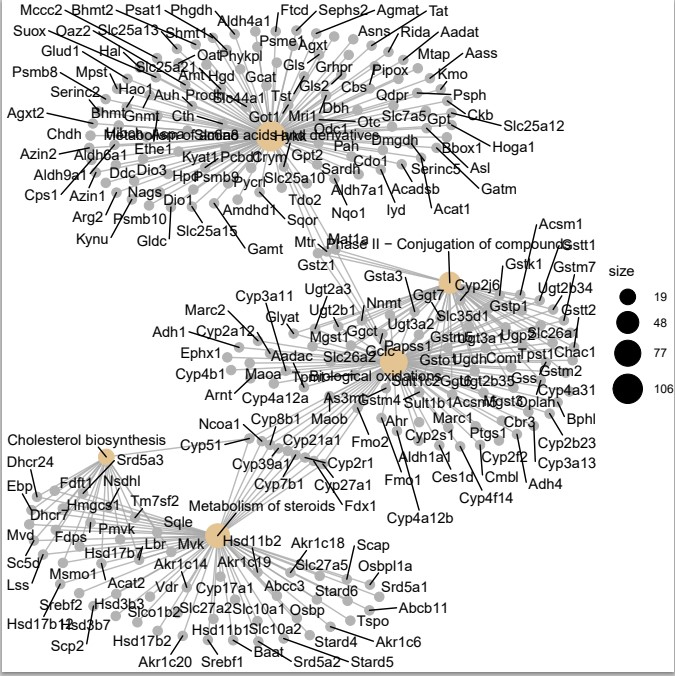
\includegraphics[width=0.75\linewidth]{figures/CNETcav} 

}

\caption{Figura 19.CNETplot de los hepatocitos con caveolina}\label{fig:CNETplotCAV}
\end{figure}

\begin{figure}

{\centering 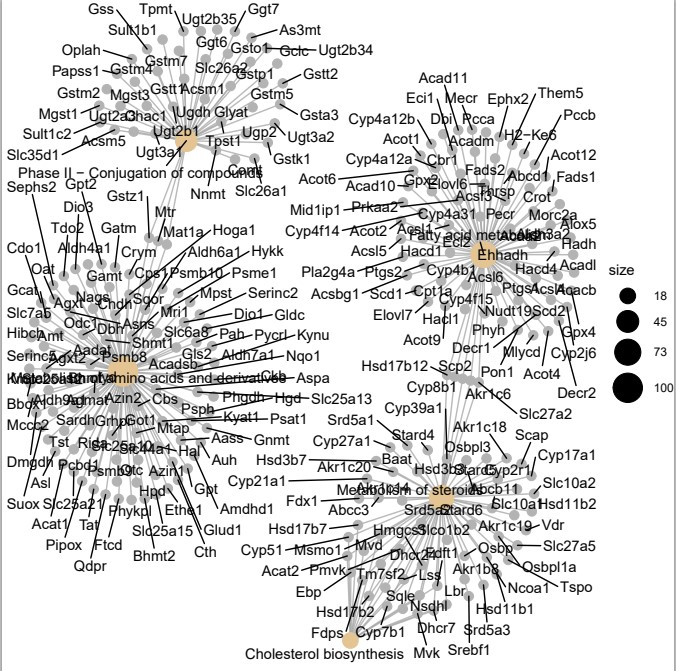
\includegraphics[width=0.75\linewidth]{figures/CNETcon} 

}

\caption{Figura 20.CNETplot de expresión génica de los hepatocitos sin caveolina}\label{fig:CNETplotCON}
\end{figure}

\begin{figure}

{\centering \includegraphics{cartoixa_david_ADO_PEC1_files/figure-latex/summary-1} 

}

\caption{Figura 21. Red de los 20 términos GO más relevantes para CAV}\label{fig:summary}
\end{figure}

En la figura 21 visualizamos el análisis de enriquecimiento visto de una
manera diferente, mediante un heatplot el cual es parecido a un cnetplot
pero mucho más visual, se muestran las 20 vias más relevantes de Gene
Ontology.

En las dos tablas siguientes se muestran las vias más relevantes para
las comparaciones CAV y CON, mostramos las primeras 5 lineas:

\begin{table}

\caption{\label{tab:summary2}Primeras filas y columnas para la comparacion CAV}
\centering
\begin{tabular}[t]{llllll}
\toprule
  & Description & GeneRatio & BgRatio & pvalue & p.adjust\\
\midrule
R-MMU-71291 & Metabolism of amino acids and derivatives & 106/2241 & 249/8772 & 2.20623045495775e-09 & 2.29889213406597e-06\\
R-MMU-8957322 & Metabolism of steroids & 61/2241 & 125/8772 & 1.54647735227951e-08 & 8.05714700537623e-06\\
R-MMU-191273 & Cholesterol biosynthesis & 19/2241 & 25/8772 & 1.75938777029171e-07 & 6.11094018881319e-05\\
R-MMU-156580 & Phase II - Conjugation of compounds & 44/2241 & 88/8772 & 6.57396625522371e-07 & 0.000140683363370677\\
R-MMU-211859 & Biological oxidations & 83/2241 & 202/8772 & 7.52179247770328e-07 & 0.000140683363370677\\
\bottomrule
\end{tabular}
\end{table}

\begin{table}

\caption{\label{tab:summary3}Primeras filas y columnas para la comparacion CON}
\centering
\begin{tabular}[t]{llllll}
\toprule
  & Description & GeneRatio & BgRatio & pvalue & p.adjust\\
\midrule
R-MMU-8957322 & Metabolism of steroids & 61/2175 & 125/8772 & 4.55505489760112e-09 & 4.72359192881236e-06\\
R-MMU-71291 & Metabolism of amino acids and derivatives & 100/2175 & 249/8772 & 4.36397779980559e-08 & 2.2627224891992e-05\\
R-MMU-8978868 & Fatty acid metabolism & 72/2175 & 169/8772 & 2.3549474272351e-07 & 8.140268273476e-05\\
R-MMU-156580 & Phase II - Conjugation of compounds & 43/2175 & 88/8772 & 8.17764037688801e-07 & 0.000155763233681676\\
R-MMU-191273 & Cholesterol biosynthesis & 18/2175 & 25/8772 & 8.93978148867076e-07 & 0.000155763233681676\\
\bottomrule
\end{tabular}
\end{table}

\hypertarget{cuxf3digo-r}{%
\section{4. Código R}\label{cuxf3digo-r}}

Debido a la extensión del código no se ha mostrado en su totalidad en el
archivo en pdf, está recopilado íntegramente como apéndice en el archivo
rcode.txt en la carpeta results y además está disponible en su totalidad
en el archivo cartoixa\_david\_ADO\_PEC1.rmd

\hypertarget{referencias}{%
\section{5. Referencias}\label{referencias}}

Ricardo Gonzalo, Sanchez-Pla A. Statistical analysis of microarray data
2019.
\url{https://github.com/ASPteaching/Omics_Data_Analysis-Case_Study_1-Microarrays}

Mei Han, Zeribe Chike Nwosu, Weronika Pooronska, Matthias Philip Ebert,
Steven Dooley, Christoph Meyer. Caveolin-1 Impacts on TGFBetha
Regulation of Metabolic Gene Signatures in Hepatocytes. Front Physiol.
2020 Jan 21;10:1606.doi:10.3389/fphys.2019.01606.eCollection 2019.

\end{document}
